\documentclass{article}

% Named technical report (not an anonymous NeurIPS submission).
% On Overleaf: if the official NeurIPS 2024 template is used, keep *their*
% neurips_2024.sty and delete the local copy if they conflict.
\usepackage[preprint]{neurips_2024}

\usepackage{amsmath,amssymb,amsthm}
\usepackage{booktabs}
\usepackage{tabularx}
\usepackage{array}
\usepackage{graphicx}
\usepackage{subcaption}
\usepackage{tikz}
\usepackage{float}
\usepackage{hyperref}
\usepackage{cleveref}
\usepackage{microtype}

\usetikzlibrary{arrows.meta,positioning,calc,fit,shapes.geometric}

\hypersetup{
  colorlinks=true,
  linkcolor=blue!50!black,
  citecolor=blue!50!black,
  urlcolor=blue!50!black
}

% Shorthand used across sections. Keep notation consistent.
\newcommand{\xlr}{x_{\mathrm{lr}}}
\newcommand{\xhr}{x_{\mathrm{hr}}}
\newcommand{\zlr}{z_{\mathrm{lr}}}
\newcommand{\zhr}{z_{\mathrm{hr}}}
\newcommand{\zsr}{z_{\mathrm{sr}}}
\newcommand{\zt}{z_{t}}
\newcommand{\zhat}{\hat{z}_{0}}
\newcommand{\xup}{x_{\mathrm{lr}}^{\uparrow}}
\newcommand{\Enc}{E}
\newcommand{\Dec}{D}
\newcommand{\vaeone}{\textsc{VAE-1}}
\newcommand{\vaesr}{\textsc{VAE-SR}}
\newcommand{\lsrmethod}{\textsc{LatentSR}}
\newcommand{\lamg}{\lambda_{g}}
\newcommand{\lamal}{\lambda_{\mathrm{align}}}
\newcommand{\sg}{\operatorname{sg}}
\newcommand{\Ebb}{\mathbb{E}}
\newcommand{\Rbb}{\mathbb{R}}
\newcommand{\Ncal}{\mathcal{N}}
\newcommand{\Lcal}{\mathcal{L}}
\newcommand{\eps}{\varepsilon}
\newcommand{\epshat}{\hat{\varepsilon}}
\newcommand{\abart}{\bar{\alpha}_{t}}


\title{When Does Better Conditioning Help?\\
Representation, Injection, and Sampling-Time Guidance\\
in Latent Diffusion Super-Resolution}

\author{%
  Hussein Hamouda \\
  Purdue University \\
  \texttt{hanafy@purdue.edu}
}

\begin{document}

\maketitle

\begin{abstract}
Latent diffusion super-resolution (SR) conditions a reverse process on a
low-resolution (LR) latent~$\zlr$.
A natural hypothesis is that a better~$\zlr$ should yield better SR.
We test that hypothesis under a controlled $4\times$ CelebA protocol
($32\!\to\!128$) with matched denoisers, frozen autoencoders, and
per-image reverse-process noise.
An SR-aware VAE improves the LR code substantially:
soft-decode $\Dec(\zlr)$ gains $\mathbf{+2.33}$\,dB PSNR and LPIPS
$0.273\!\to\!0.119$ ($n{=}64$), while HR reconstruction stays at
$\approx 37.3$\,dB.
The same gain does \emph{not} transfer through a concat latent DDPM:
SR PSNR moves only $\mathbf{+0.22}$\,dB and LPIPS is a null
($\approx 0.068$); imagewise Spearman $\rho(\Delta\mathrm{soft},\Delta\mathrm{SR})\approx 0.05$.
Replacing concat with spatial FiLM is also a null
(PSNR $\Delta=-0.03$\,dB, CI includes~$0$).
A timestep diagnostic localizes the failure: the SR-aware model
becomes strongly aligned with~$\zlr$ mid-reverse (cosine $0.985$ at
$t{=}656$) and subsequently loses this alignment as sampling
approaches the final HR latent.
Inference-time decoder-side LR-consistency guidance, applied in the
late sampling window $t\le 500$ (no training), recovers
$\mathbf{56\%}$ of the $2.08$\,dB transfer gap at $\lamg{=}200$
($n{=}256$: $26.33\!\to\!27.50$\,dB) and slightly \emph{improves}
LPIPS relative to the unguided baseline ($0.0720\!\to\!0.0707$).
Our contribution is a controlled diagnosis of conditioning transfer in
latent diffusion SR and an inference-time intervention that recovers a
substantial fraction of the lost fidelity.

\end{abstract}

\section{Introduction}
\label{sec:intro}

Generative super-resolution (SR) increasingly runs in a
\emph{latent} space: an autoencoder compresses images, a diffusion
model denoises the high-resolution (HR) latent, and a decoder returns
pixels~\citep{rombach2022high,saharia2023image,wang2024exploiting}.
The low-resolution (LR) observation enters as a condition, typically
the encoded upsampled LR image $\zlr=\Enc(\xup)$.
This design assumes a convenient causal story:
if $\zlr$ is a better representation of the HR target, the reverse
process should emit a better $\zsr$, and SR metrics should follow.

That story is not a theorem.
It confuses two jobs that share a decoder but not an objective
(\Cref{tab:two-jobs}):
soft-decode $\Dec(\zlr)$ scores what is already in the LR code;
\lsrmethod{} $\Dec(\zsr)$ scores what a conditional DDPM uses while
sampling $p(\zhr\mid\zlr)$.

This paper is a controlled diagnosis of that transfer, not a new
SOTA SR method.
We freeze the data, the UNet skeleton, the noise schedule, and the
evaluation noise, and change one link at a time
(\Cref{fig:causal-chain}): representation (\vaesr), injection
(concat vs.\ spatial FiLM), reverse-chain measurement, then
inference-time LR-consistency guidance.
Headline outcomes---a large soft-decode gain that concat and FiLM
do not consume, a mid-reverse copy that later collapses, and late
guidance that recovers about half the gap---are in~\S\ref{sec:experiments}.
The intervention that works is not the one the representation
hypothesis suggested.

\paragraph{Scope.}
No new backbone, tokenizer, or trained guidance network.
The FiLM null is for this conditioner on this frozen \vaesr{} code.
$\Dec(\zlr)$ is not an SR method.
Citation hygiene:~\S\ref{sec:setup-hygiene}.

\begin{figure*}[t]
  \centering
  \resizebox{\textwidth}{!}{%
  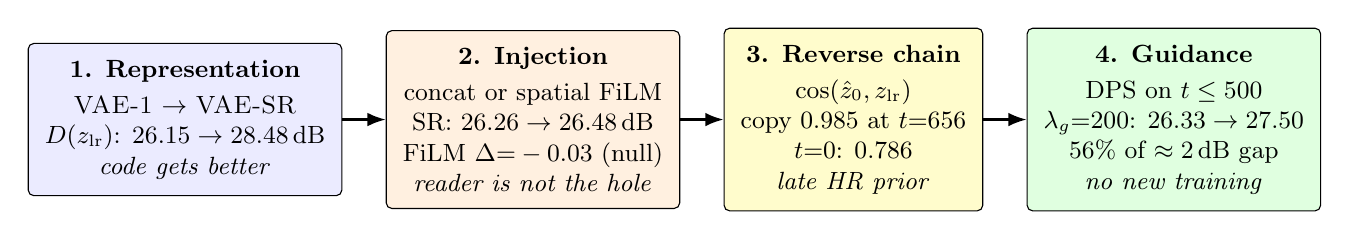
\begin{tikzpicture}[
      font=\small,
      box/.style={draw, rounded corners=2pt, align=center, inner sep=6pt, minimum height=1.35cm},
      arr/.style={-{Latex}, thick}
    ]
    \node[box, fill=blue!8] (rep) {%
      \textbf{1. Representation}\\[2pt]
      \vaeone{} $\to$ \vaesr\\
      $\Dec(\zlr)$: $26.15\to 28.48$\,dB\\
      \textit{code gets better}};
    \node[box, fill=orange!12, right=0.55cm of rep] (inj) {%
      \textbf{2. Injection}\\[2pt]
      concat or spatial FiLM\\
      SR: $26.26\to 26.48$\,dB\\
      FiLM $\Delta{=}-0.03$ (null)\\
      \textit{reader is not the hole}};
    \node[box, fill=yellow!20, right=0.55cm of inj] (traj) {%
      \textbf{3. Reverse chain}\\[2pt]
      $\cos(\zhat,\zlr)$\\
      copy $0.985$ at $t{=}656$\\
      $t{=}0$: $0.786$\\
      \textit{late HR prior}};
    \node[box, fill=green!12, right=0.55cm of traj] (guid) {%
      \textbf{4. Guidance}\\[2pt]
      DPS on $t\le 500$\\
      $\lamg{=}200$: $26.33\to 27.50$\\
      $56\%$ of $\approx 2$\,dB gap\\
      \textit{no new training}};
    \draw[arr] (rep) -- (inj);
    \draw[arr] (inj) -- (traj);
    \draw[arr] (traj) -- (guid);
  \end{tikzpicture}%
  }
  \caption{Causal chain.
  Each box changes one link and holds the others fixed.
  Numbers are the locked outcomes of~\S\ref{sec:experiments}
  ($n{=}64$ except the last box, which is the $n{=}256$ dose).}
  \label{fig:causal-chain}
\end{figure*}

\section{Problem setup and pipeline}
\label{sec:setup}

This section fixes notation, the two decode jobs, the data and
denoiser, and the evaluation protocol used by every later table.
Method variants (\vaeone{} vs.\ \vaesr, concat vs.\ FiLM, guidance)
are defined in~\S\ref{sec:setup}--\S\ref{sec:setup-hygiene} only as
\emph{interfaces}; training losses and ablations come in subsequent
sections.

\subsection{Task and notation}
\label{sec:notation}

Let $\xhr\in\Rbb^{3\times 128\times 128}$ be an HR RGB face and
$\xlr\in\Rbb^{3\times 32\times 32}$ its $4\times$ bicubic
downsample.
Write $\xup$ for bicubic upsample of $\xlr$ back to $128\times 128$.
A convolutional VAE provides an encoder--decoder pair
$(\Enc,\Dec)$ with spatial latent shape $(4,32,32)$ (downsample
factor~$4$).
The encoder outputs a diagonal Gaussian
$q(z\mid x)=\Ncal(\mu(x),\mathrm{diag}(\sigma^2(x)))$.
At SR inference we freeze the VAE and use the posterior
\emph{mean}
\begin{equation}
  \label{eq:latent-mean}
  z \;=\; \mu(x),\qquad
  z_{\mathrm{scaled}} \;=\; s\,z,\qquad
  \Dec_{\mathrm{scaled}}(z) \;=\; \Dec(z/s),
\end{equation}
with $s{=}1$ throughout (a scale $1/\mathrm{std}(\mu_{\mathrm{hr}})\approx 1.065$
was estimated and \emph{not} applied).

The diffusion model is a DDPM~\citep{ho2020denoising} on the HR
latent $\zhr=\Enc(\xhr)$, with $T{=}1000$ steps and a linear
schedule $\beta_t\in[10^{-4},0.02]$.
We write $\abart=\prod_{s=1}^{t}\alpha_s$ in the usual way.
The UNet predicts noise $\epshat_\theta(\zt,\zlr,t)$.
The predicted clean latent is
\begin{equation}
  \label{eq:z0hat}
  \zhat(t)
  \;=\;
  \frac{\zt - \sqrt{1-\abart}\,\epshat_\theta(\zt,\zlr,t)}{\sqrt{\abart}}.
\end{equation}
Reverse sampling uses the standard DDPM posterior step
$p(z_{t-1}\mid \zt,\epshat)$.
The SR output is $\zsr\approx z_0$ after $t{=}0$, decoded as
$\Dec(\zsr)$.

\paragraph{Two decodes.}
\Cref{tab:two-jobs} is the wording constraint for the rest of the
paper.
Soft-decode reconstructs the \emph{condition}.
\lsrmethod{} samples an HR latent.
We never say that the DDPM ``overwrites a better reconstruction.''

\begin{table}[htbp]
  \centering
  \caption{Two jobs that share $\Dec$ but not an objective.}
  \label{tab:two-jobs}
  \small
  \setlength{\tabcolsep}{3pt}
  \begin{tabularx}{\columnwidth}{@{}
      >{\raggedright\arraybackslash}p{1.55cm}
      >{\raggedright\arraybackslash}X
      >{\raggedright\arraybackslash}X@{}}
    \toprule
    Name & Definition & Question \\
    \midrule
    Soft-decode &
      $\Dec(\zlr)=\Dec(\Enc(\xup))$ &
      What HR-looking information is already in $\zlr$? \\
    \lsrmethod{} &
      $\Dec(\zsr)$, $\zsr\sim p(\zhr\mid\zlr)$ &
      How much of that information does the sampler use? \\
    \bottomrule
  \end{tabularx}
\end{table}

\subsection{Data, architecture, and training constants}
\label{sec:data}

\begin{table}[htbp]
  \centering
  \caption{Locked experimental constants. Changing any row without
  a paired re-eval invalidates a comparison.}
  \label{tab:constants}
  \small
  \setlength{\tabcolsep}{4pt}
  \begin{tabularx}{\columnwidth}{@{}lX@{}}
    \toprule
    Item & Value \\
    \midrule
    Dataset & CelebA, center-crop $178$, then resize \\
    HR / LR & $128\times 128$ / $32\times 32$ ($4\times$ bicubic) \\
    Valid split & official; eval in file order, $\texttt{shuffle=False}$ \\
    Valid size & $\approx 19{,}867$ (full val never run) \\
    Seed & $42$; $x_T$ and every reverse-step noise seeded per \texttt{val\_index} \\
    VAE & conv.\ $\beta$-VAE, base channels $64$, \texttt{channel\_mult}$=[1,2,4]$, $2$ resblocks \\
    Latent & $(4,32,32)$, $s{=}1$ \\
    DDPM & $T{=}1000$, $\beta\in[10^{-4},0.02]$, Adam $2{\times}10^{-4}$ \\
    UNet & same skeleton as the VAE width, attn.\ at $16$ and $8$ \\
    Concat DDPM & $50$ epochs, batch $64$ \\
    \bottomrule
  \end{tabularx}
\end{table}

\Cref{tab:constants} lists the constants that never change across
the causal chain.
CelebA faces keep the problem in a well-understood, aligned domain;
the point is isolation, not real-world degradation modeling.
The denoiser is the project's own latent UNet
(\texttt{generative\_models.ddpm}), not a pretrained Stable Diffusion
backbone, so representation, injection, and sampling effects are not
confounded with a frozen billion-parameter prior.

\subsection{Pipeline}
\label{sec:pipeline}

\Cref{fig:pipeline} is the system at inference.
HR and LR share one frozen encoder.
The denoiser never sees pixels: it sees $\zt$ and $\zlr$ only.
Conditioning is either channel concat
\begin{equation}
  \label{eq:concat}
  \epshat_\theta(\zt,\zlr,t)
  \;=\;
  \mathrm{UNet}\bigl([\zt \,\Vert\, \zlr],\, t\bigr)
\end{equation}
($8$ input channels, $4$ output channels) or spatial FiLM at every
UNet scale (defined when that experiment is introduced).
Guidance, when used, does not change~\eqref{eq:concat}: it adds a
decoder-side correction after the unguided posterior step
(\S\ref{sec:method-guide}).

\begin{figure*}[t]
  \centering
  \resizebox{0.98\textwidth}{!}{%
  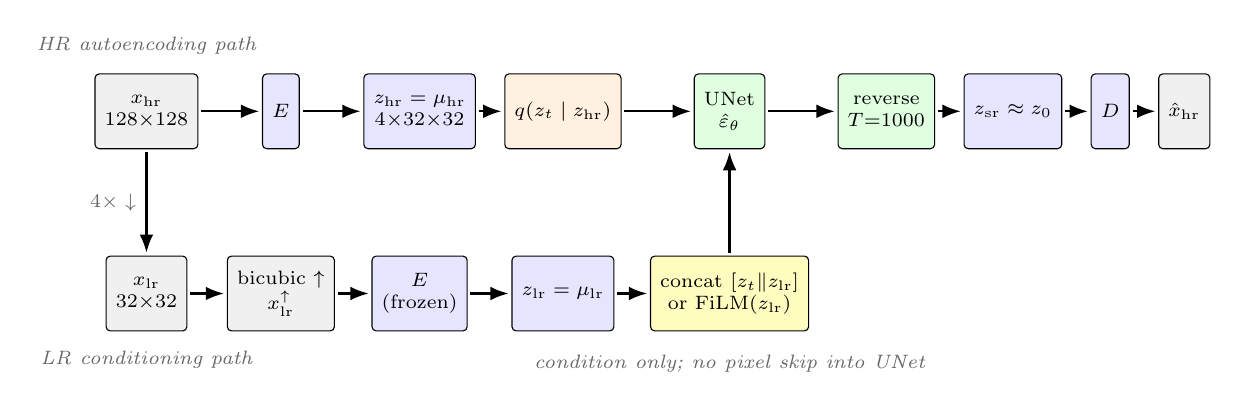
\begin{tikzpicture}[
      font=\scriptsize,
      blk/.style={draw, rounded corners=1.5pt, align=center,
                  inner sep=3.5pt, minimum height=9.5mm, anchor=center},
      lab/.style={font=\scriptsize\itshape, text=black!60},
      arr/.style={-{Latex}, thick, shorten >=1pt, shorten <=1pt}
    ]
    \matrix[
      ampersand replacement=\&,
      column sep=3.6mm,
      row sep=1.35cm,
      cells={anchor=center, inner sep=0pt}
    ] {
      \node[blk, fill=gray!12] (xhr) {$\xhr$\\$128{\times}128$}; \&
      \node[blk, fill=blue!10] (ehr) {$\Enc$}; \&
      \node[blk, fill=blue!10] (zhr) {$\zhr=\mu_{\mathrm{hr}}$\\$4{\times}32{\times}32$}; \&
      \node[blk, fill=orange!12] (fwd) {$q(\zt\mid\zhr)$}; \&
      \node[blk, fill=green!12] (unet) {UNet\\$\epshat_\theta$}; \&
      \node[blk, fill=green!12] (rev) {reverse\\$T{=}1000$}; \&
      \node[blk, fill=blue!10] (zsr) {$\zsr\approx z_0$}; \&
      \node[blk, fill=blue!10] (dec) {$\Dec$}; \&
      \node[blk, fill=gray!12] (out) {$\hat x_{\mathrm{hr}}$}; \\
      \node[blk, fill=gray!12] (xlr) {$\xlr$\\$32{\times}32$}; \&
      \node[blk, fill=gray!12] (up) {bicubic $\uparrow$\\$\xup$}; \&
      \node[blk, fill=blue!10] (elr) {$\Enc$\\(frozen)}; \&
      \node[blk, fill=blue!10] (zlr) {$\zlr=\mu_{\mathrm{lr}}$}; \&
      \node[blk, fill=yellow!25] (cond) {concat $[\zt\Vert\zlr]$\\or FiLM$(\zlr)$}; \\
    };

    \draw[arr] (xhr) -- (ehr);
    \draw[arr] (ehr) -- (zhr);
    \draw[arr] (zhr) -- (fwd);
    \draw[arr] (fwd) -- (unet);
    \draw[arr] (unet) -- (rev);
    \draw[arr] (rev) -- (zsr);
    \draw[arr] (zsr) -- (dec);
    \draw[arr] (dec) -- (out);

    \draw[arr] (xhr) -- node[left, lab] {$4\times\downarrow$} (xlr);
    \draw[arr] (xlr) -- (up);
    \draw[arr] (up) -- (elr);
    \draw[arr] (elr) -- (zlr);
    \draw[arr] (zlr) -- (cond);
    % Conditioning enters the UNet from below (not a leftward hook).
    \draw[arr] (cond.north) -- (unet.south);

    \node[lab, below=0.18cm of cond] {condition only; no pixel skip into UNet};
    \node[lab, above=0.12cm of xhr] {HR autoencoding path};
    \node[lab, below=0.12cm of xlr] {LR conditioning path};
  \end{tikzpicture}%
  }
  \caption{LatentSR inference pipeline (every stage that later tables
  refer to).
  Blue: frozen VAE.
  Orange: forward diffusion on $\zhr$ (training) / noise at $t{=}T$ (eval).
  Green: concat or FiLM denoiser.
  Yellow: the only place the LR code enters the UNet.
  Soft-decode is $\Dec(\zlr)$ and never uses the green path.
  \lsrmethod{} is $\Dec(\zsr)$.}
  \label{fig:pipeline}
\end{figure*}

\subsection{Evaluation protocol}
\label{sec:eval}

Every paired claim uses the same $N$ CelebA validation images in file
order, seed~$42$, and reverse-process noise drawn as a function of
\texttt{val\_index}.
Two checkpoints are therefore comparable even if batch size differs.
Primary metrics are PSNR (distortion) and LPIPS-Alex
\citep{zhang2018unreasonable} (perception).
SSIM and Sobel edge MAE are secondary.
Paired tests: $\Delta$ is candidate minus baseline on matched
indices; sign-flip permutation $n_{\mathrm{perm}}{=}10^{4}$;
percentile bootstrap $95\%$ CI $n_{\mathrm{boot}}{=}10^{4}$.
We declare a mean $\Delta$ real when the CI excludes $0$.

\paragraph{Number hygiene.}
VAE, concat, FiLM, timestep, and $\zhat$-image diagnostics are
reported at $\mathbf{n{=}64}$.
The guidance \emph{dose} that we treat as confirmatory is
$\mathbf{n{=}256}$ (\texttt{val\_index} $0..255$), pre-registered
before looking at those numbers.
We never pool the two $n$ in one mean.
Full validation ($\approx 19{,}867$) is not computationally feasible
at $\approx 21$\,s/image for guided reverse sampling.

\subsection{Checkpoint pairing and hygiene}
\label{sec:setup-hygiene}

Three frozen VAEs / DDPMs are easy to mix because several artifacts
are named \texttt{latest.pt}.
\Cref{tab:ckpts} is the pairing used in every later section.
Guidance is always Q2 concat epoch-$50$ \emph{with} \vaesr{}
epoch-$20$.
Phase-8 concat (trained on \vaeone) and the FiLM checkpoint are
never used for guidance.

\begin{table}[htbp]
  \centering
  \caption{Checkpoint pairing used in every later section.}
  \label{tab:ckpts}
  \small
  \setlength{\tabcolsep}{4pt}
  \begin{tabularx}{\columnwidth}{@{}lXX@{}}
    \toprule
    Name & Frozen VAE & Role \\
    \midrule
    \vaeone{} & recon.\ VAE, epoch $50$ & representation baseline \\
    \vaesr{} & $20$-epoch align fine-tune & representation test \\
    Phase-8 concat & \vaeone{} & not for guidance \\
    Q2 concat & \vaesr{} & transfer + guidance pair \\
    FiLM Q2 & \vaesr{} & injection test only \\
    \bottomrule
  \end{tabularx}
\end{table}

\paragraph{Citation hygiene.}
On $2026$-$08$-$19$ a related-work list named a paper as
``PGSR --- When Latents Forget Pixels ($2026$)'' without authors,
arXiv ID, venue, or DOI.
The acronym collides with planar-based Gaussian splatting; a
circulating code URL did not check out as that SR paper.
We exclude it: a title-plus-year string is not a citation.

\section{Related work}
\label{sec:related}

We group prior work by the three links we ablate---how $\zlr$ is
\emph{represented}, how it is \emph{injected} into a denoiser, and
how sampling can be \emph{steered} back toward the LR
observation---and then state what is \emph{not} claimed.

\subsection{Latent diffusion and generative SR}
Denoising diffusion~\citep{ho2020denoising} produces high-quality
images by reversing a Gaussian noising process.
Latent diffusion~\citep{rombach2022high} moves that process into the
code of a convolutional VAE~\citep{kingma2014auto}, which is the
template for \lsrmethod{}: encode, denoise, decode.
Pixel-space iterative SR~\citep{saharia2023image} showed that a
conditional DDPM can outperform regression on perceptual metrics;
subsequent systems adapt large pretrained latent priors for
restoration, including StableSR~\citep{wang2024exploiting},
DiffBIR~\citep{lin2024diffbir}, and
SeeSR~\citep{wu2024seesr}.
Those methods are engineering stacks (ControlNet branches, semantic
prompts, degradation-aware encoders) on frozen billion-parameter
backbones.
Our denoiser is a small latent UNet trained from scratch on
CelebA~\citep{liu2015faceattributes}, on purpose:
representation, injection, and sampling can be swapped without
confounding a pretrained generative prior.

The perception--distortion trade-off~\citep{blau2018perception} is
the right backdrop for every SR table below.
LPIPS~\citep{zhang2018unreasonable} tracks the perceptual axis;
PSNR tracks distortion.
A method can win LPIPS while losing PSNR, and a soft-decode that
looks closer to HR than the sampler's output is not a bug in the
metrics.

\subsection{Representations for restoration}
A reconstruction VAE is optimized for $\Dec(\zhr)\approx\xhr$, not
for $\zlr$ to be a useful SR condition.
Related restoration work often adds pixel-space skip connections,
second encoders, or pretrained tokenizers.
We stay inside one frozen VAE so that ``better $\zlr$'' is a measured
change in $\Dec(\zlr)$ and cosine$(\zlr,\zhr)$---not a new
architecture.
The hypothesis we test is the one implicit in much latent SR:
if those representation metrics improve, SR metrics should follow.

\subsection{How the LR code is injected}
The default in latent SR, and our baseline, is channel concat
$[\zt\Vert\zlr]$ at the UNet input~\citep{rombach2022high}.
Concat is spatially aligned---our $\zlr$ is already $4\times 32\times 32$---but
it touches only the first convolution.
Feature-wise modulation (FiLM;~\citealp{perez2018film}) and its
normalization cousins (AdaIN/AdaGN) inject a condition as
$\gamma,\beta$ at many depths, the natural test of
``concat cannot read $\zlr$ after the first conv.''
ControlNet-style side branches~\citep{zhang2023adding} and
cross-attention are the other common readers.
We use neither: cross-attention would treat an already-aligned map as
tokens, and ControlNet would add a second encoder.
A FiLM null on the same frozen $\zlr$ is evidence against the
weak-reader story, not a claim that FiLM never helps in other stacks.

\subsection{Sampling-time guidance and prior vs.\ fidelity}
Classifier guidance~\citep{dhariwal2021diffusion} and classifier-free
guidance~\citep{ho2022classifier} steer a reverse process with a
gradient or a conditional/unconditional pair.
Diffusion posterior sampling
(DPS;~\citealp{chung2023diffusion}) applies a measurement gradient
through a differentiable forward model, typically to $z_{t-1}$ after
an unguided posterior step.
SeeSR~\citep{wu2024seesr} and DiffBIR~\citep{lin2024diffbir}
discuss generative priors that invent plausible but unfaithful
detail; they add semantic or restoration conditions during sampling
or via extra trained modules.
Our probe uses that DPS pattern with an LR-consistency measurement
through a frozen decoder, in a pre-registered time window, with
$\lamg$ chosen from a relative step size $R(t)$ rather than from a
test-set sweep disguised as a method (\S\ref{sec:method-guide}).

\subsection{Positioning}
The experiment is narrow: hold the denoiser family and evaluation
noise fixed, improve $\zlr$ by a known amount, and ask whether
concat, then FiLM, then late-window guidance consume that gain.
We do not claim a new conditioning architecture or reproduce
large-prior pipelines.
A claimed related paper could not be verified from the citation as
given and is excluded (\S\ref{sec:setup-hygiene}).

\section{Method}
\label{sec:method}

We change one link of \Cref{fig:pipeline} at a time.
This section specifies the four interventions---representation,
injection, trajectory measurement, and sampling-time
guidance---before any SR table.
Training hyperparameters that never change are in
\Cref{tab:constants}; checkpoint pairing is in \Cref{tab:ckpts}.

\subsection{Stage A: reconstruction VAE (\vaeone)}
\label{sec:method-vae1}

\vaeone{} is a convolutional $\beta$-VAE~\citep{kingma2014auto}
trained only to reconstruct HR CelebA faces.
It has no SR term.
The encoder outputs $(\mu,\log\sigma^2)$; training uses
$z=\mu+\sigma\odot\eps$ with $\eps\sim\Ncal(0,I)$.
The loss is mean-reduced MSE plus a mean-reduced KL, so the KL
scale stays stable at latent size $4\times 32\times 32$:
\begin{equation}
  \label{eq:vae1}
  \begin{aligned}
    \Lcal_{\mathrm{VAE\text{-}1}}
    \;=\;
    &\underbrace{\lVert \Dec(z)-\xhr\rVert_2^2}_{\Lcal_{\mathrm{recon}}} \\
    &+\beta\,
    \underbrace{\Ebb\bigl[-\tfrac12\bigl(1+\log\sigma^2-\mu^2-\sigma^2\bigr)\bigr]
    }_{\mathrm{KL}},
  \end{aligned}
\end{equation}
with $\beta=10^{-4}$ and
$\mathrm{KL}=\mathrm{KL}\bigl(q(z\mid\xhr)\,\Vert\,\Ncal(0,I)\bigr)$.
We train for $50$ epochs (Adam $10^{-4}$, batch $64$) and freeze
epoch~$50$ for every later experiment.
Eval reconstructions use $\mu$, not a posterior sample.

\subsection{Stage B: SR-aware alignment (\vaesr)}
\label{sec:method-vaesr}

\vaesr{} is \vaeone{} fine-tuned so the LR encoder mean moves toward
the HR encoder mean without rebuilding the autoencoder
(\Cref{fig:stage-vae}).
Initialize from \vaeone{} epoch~$50$.
On each batch encode HR and the bicubic-upsampled LR with the
\emph{same} encoder
\begin{equation}
  \label{eq:mu-pair}
  \mu_{\mathrm{hr}},\log\sigma^2_{\mathrm{hr}} \;=\; \Enc(\xhr),\qquad
  \mu_{\mathrm{lr}} \;=\; \Enc(\xup),
\end{equation}
and optimize
\begin{equation}
  \label{eq:vaesr}
  \begin{aligned}
    \Lcal_{\mathrm{VAE\text{-}SR}}
    \;=\;
    &\Lcal_{\mathrm{recon}}(\xhr,\Dec(z_{\mathrm{hr}})) \\
    &+\beta\,\mathrm{KL}\bigl(q(z\mid\xhr)\,\Vert\,\Ncal(0,I)\bigr) \\
    &+\lamal \lVert \mu_{\mathrm{lr}} - \sg(\mu_{\mathrm{hr}}) \rVert_2^2.
  \end{aligned}
\end{equation}
Stop-gradient $\sg(\cdot)$ on $\mu_{\mathrm{hr}}$ is required: without
it the HR code can collapse toward the blurry LR code; with it, only
the LR mean is pulled.
$\beta$ is unchanged ($10^{-4}$).
$\lamal=10^{-3}$ because unweighted align MSE starts near $0.58$;
$10^{-3}$ keeps the term on the order of recon MSE.
We fine-tune for $20$ epochs (Adam $10^{-4}$, batch $32$) and freeze
the result.
A $\lamal$ sweep is \emph{not} part of the method: cosine$(\zlr,\zhr)$
plateaus after epoch~$1$, so the next causal question is consumption,
not more alignment.

\begin{figure}[htbp]
  \centering
  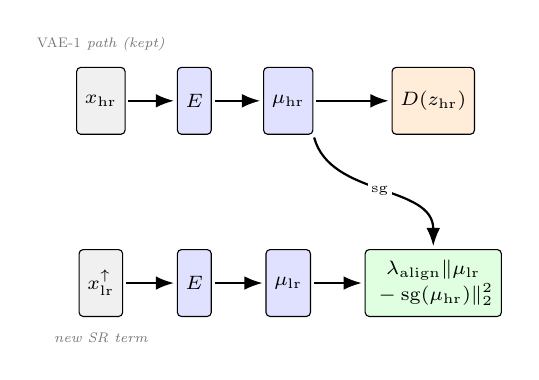
\begin{tikzpicture}[
      font=\scriptsize,
      blk/.style={draw, rounded corners=1.5pt, align=center, inner sep=3pt,
                  minimum height=8.5mm, anchor=center},
      arr/.style={-{Latex}, thick, shorten >=1pt, shorten <=1pt}
    ]
    \matrix[
      ampersand replacement=\&,
      column sep=6.5mm,
      row sep=1.45cm,
      cells={anchor=center, inner sep=0pt}
    ] {
      \node[blk, fill=gray!12] (hr) {$\xhr$}; \&
      \node[blk, fill=blue!12] (ehr) {$\Enc$}; \&
      \node[blk, fill=blue!12] (muh) {$\mu_{\mathrm{hr}}$}; \&
      \node[blk, fill=orange!15] (dec) {$\Dec(z_{\mathrm{hr}})$}; \\
      \node[blk, fill=gray!12] (lr) {$\xup$}; \&
      \node[blk, fill=blue!12] (elr) {$\Enc$}; \&
      \node[blk, fill=blue!12] (mul) {$\mu_{\mathrm{lr}}$}; \&
      \node[blk, fill=green!12] (aln) {$\lamal\lVert\mu_{\mathrm{lr}}$\\
        ${}-\sg(\mu_{\mathrm{hr}})\rVert_2^2$}; \\
    };
    \draw[arr] (hr) -- (ehr);
    \draw[arr] (lr) -- (elr);
    \draw[arr] (ehr) -- (muh);
    \draw[arr] (elr) -- (mul);
    \draw[arr] (muh) -- (dec);
    \draw[arr] (mul) -- (aln);
    % Stop-grad: label sits on the arrow, not floating above it.
    \draw[arr] (muh.south east) to[out=-75, in=90]
      node[pos=0.5, fill=white, inner sep=1.2pt, font=\tiny] {$\sg$} (aln.north);
    \node[font=\tiny\itshape, text=black!55, above=0.08cm of hr] {\vaeone{} path (kept)};
    \node[font=\tiny\itshape, text=black!55, below=0.08cm of lr] {new SR term};
  \end{tikzpicture}
  \caption{\vaesr{} fine-tune.
  HR recon+KL is the \vaeone{} loss~\eqref{eq:vae1}.
  Alignment pulls $\mu_{\mathrm{lr}}$ toward a stop-grad $\mu_{\mathrm{hr}}$.
  Soft-decode later scores $\Dec(\mu_{\mathrm{lr}})$, not this training grid.}
  \label{fig:stage-vae}
\end{figure}

\subsection{Stage C: concat latent DDPM}
\label{sec:method-concat}

Given a frozen VAE, we train a noise-prediction UNet on
$z_{\mathrm{hr}}$ with channel-concat conditioning~\eqref{eq:concat}:
eight input channels, four output channels, same skeleton and
$50$-epoch recipe for both VAEs.
The training loss is standard DDPM noise MSE~\citep{ho2020denoising}.
Only the frozen VAE changes between the \vaeone{} concat run
(Phase~8) and the \vaesr{} concat run (Q2).
We do not resume a concat checkpoint into FiLM (channel layout
differs).

\subsection{Stage D: spatial FiLM}
\label{sec:method-film}

To test whether concat is a weak reader of an already-better
$\zlr$, we replace~\eqref{eq:concat} with spatial FiLM
\citep{perez2018film} at every UNet scale.
The noisy latent stays four channels.
At a feature map $h$ of matching (or bilinearly resized) resolution,
\begin{equation}
  \label{eq:film}
  h' \;=\; \bigl(1+\gamma(\zlr)\bigr)\odot h \;+\; \beta(\zlr),
\end{equation}
where $\gamma,\beta$ come from a $1{\times}1$ convolution that is
\emph{zero-initialized}, so the block is identity at step~$0$.
Cross-attention is not used (\S\ref{sec:related}).

\paragraph{One-sided $2{\times}2$.}
A full interaction would train FiLM on both VAEs.
With one new DDPM, we train FiLM+\vaesr{} and interpret it as a
one-sided test, written down \emph{before} seeing numbers:
if SR still matches concat+\vaesr, skip FiLM+\vaeone{} and treat
concat-as-reader as not the bottleneck;
if FiLM+\vaesr{} clearly beats concat+\vaesr, then train FiLM+\vaeone{}
before claiming an interaction.
Same $50$ epochs, same paired eval as Q2.

\subsection{Stage E: reverse-chain diagnostics}
\label{sec:method-traj}

To localize where a better $\zlr$ is or is not used, we record, at
every scheduler index $t$,
$\cos(\zhat(t),\zlr)$ and $\lVert\zhat(t)-\zlr\rVert$ under both
frozen VAEs and their matched concat DDPMs, plus the image-space
scores of $\Dec(\zhat(t))$ versus $\xhr$.
Soft-decode $\Dec(\zlr)$ is not $\Dec(\zhat(t))$ at a copy peak;
those are reported separately.

\subsection{Stage F: DPS-style LR-consistency guidance}
\label{sec:method-guide}

Guidance is inference only: frozen \vaesr{} + Q2 concat, no extra
training.
The convention is DPS-like~\citep{chung2023diffusion} and is fixed
before any guided SR number: gradient with respect to $\zt$,
correction applied to the already-sampled $z_{t-1}$.

At each reverse index $t$:
\begin{enumerate}
  \item $\epshat=\mathrm{UNet}(\zt,\zlr,t)$, \emph{detached}
        (no UNet backward).
  \item $\zhat$ as in~\eqref{eq:z0hat}.
  \item $z_{t-1}\sim p(z_{t-1}\mid \zt,\epshat)$ (unguided DDPM step).
  \item If $t$ is in the window,
\end{enumerate}
\begin{equation}
  \label{eq:guide}
  \begin{aligned}
    \Lcal_g
    &=
    \mathrm{mean}_{c,h,w}\bigl\lVert \Dec(\zhat)-\Dec(\zlr)\bigr\rVert_2^2, \\
    g
    &=
    \nabla_{\zt}\Lcal_g, \\
    z_{t-1}
    &\leftarrow
    z_{t-1}-\lamg\, g.
  \end{aligned}
\end{equation}
$\Dec(\zlr)$ is cached once per image.
Decoder weights stay frozen; the backward runs through the
$\zhat$ affine and $\Dec$ only.
Windows (scheduler index; $t{=}0$ is clean):
baseline $=$ none;
early $=$ $t\in[0,800]$ every step;
late $=$ $t\in[0,500]$ every step.
A budget skip \texttt{guide\_every}$>1$ is implemented but not used
in the reported runs.

\paragraph{Choosing $\lamg$ from $R(t)$, not from SR PSNR.}
Define the relative step size
\begin{equation}
  \label{eq:Rt}
  R(t) \;=\; \frac{\lVert g\rVert_2}{\lVert z_{t-1}-z_t\rVert_2}.
\end{equation}
A sanity sweep at $\lamg\in\{10^{-3},10^{-2},10^{-1},1\}$ gives
$R(t)<0.01$ everywhere: $\lamg{=}1$ is a no-op.
$R$ is linear in $\lamg$.
\Cref{tab:Rt} scales the $\lamg{=}1$ column.
$\lVert g\rVert/\lVert\Delta z\rVert$ drops by about $60\times$ from
$t{=}800$ to $t{=}500$, so \emph{one scalar cannot put every
checkpoint in a $0.1$--$0.5$ band}.
We take $\lamg{=}200$ as a compromise: in-band at $t{=}650$
($R{\approx}0.18$); above $0.5$ but below a $2$--$3$ dominate
ceiling at $t{=}800$ ($R{\approx}1.16$); small but non-zero in the
late window ($R(500){\approx}0.04$).
$\lamg{=}400$ would make the late window fairer but
$R(800){\approx}2.3$.
A late PSNR-null is not treated as localization failure unless
$R(t)$ for $t\le 500$ is clearly $>0$.

\begin{table}[htbp]
  \centering
  \caption{Relative guidance size $R(t)$~\eqref{eq:Rt}, scaled from
  a $\lamg{=}1$ measurement. Bold: operating column.}
  \label{tab:Rt}
  \small
  \begin{tabular}{@{}rcccc@{}}
    \toprule
    $t$ & $R(1)$ & $R(100)$ & $\mathbf{R(200)}$ & $R(400)$ \\
    \midrule
    $800$ & $0.0058$ & $0.58$ & $\mathbf{1.16}$ & $2.32$ \\
    $650$ & $0.0009$ & $0.09$ & $\mathbf{0.18}$ & $0.36$ \\
    $500$ & $0.0002$ & $0.02$ & $\mathbf{0.04}$ & $0.08$ \\
    $300$ & $0.0001$ & $0.01$ & $\mathbf{0.02}$ & $0.04$ \\
    $100$ & $0.0001$ & $0.01$ & $\mathbf{0.02}$ & $0.04$ \\
    \bottomrule
  \end{tabular}
\end{table}

\paragraph{Pre-registered calls (before guided PSNR).}
PSNR$\uparrow$ with LPIPS $\approx 0.068$ is a strong positive;
PSNR$\uparrow$ with LPIPS toward $0.119$ is over-guidance.
If both windows work, Stage~2 is a late-window dose
$\lamg\in\{50,200,800\}$ only---no combined schedule.
The $n{=}256$ confirmation (val\_index $0..255$, same checkpoints,
late window) is declared before looking at those numbers, and
survives iff (a)~$\ge 90\%$ of images have $\Delta\mathrm{PSNR}>0$ at
each $\lamg$, (b)~mean $\Delta$LPIPS is monotone
$50<200<800$ with $\lamg{=}800$ worse than unguided and
$\lamg{=}50$ not worse, (c)~PSNR CIs exclude $0$ at all three
$\lamg$.
The first line of each job must reprint
$\mathrm{PSNR}(\Dec(\zlr),\xhr)\approx 28.48$ on indices $0..63$;
otherwise the wrong VAE is loaded and the run is discarded.

\section{Experiments}
\label{sec:experiments}

Every table uses~\S\ref{sec:eval}: same \texttt{val\_index} order,
seed~$42$, reverse-process noise as a function of index, pairing
from~\Cref{tab:ckpts}.
VAE, concat, FiLM, and trajectory are $n{=}64$; the confirmatory
guidance dose is $n{=}256$.
The two $n$ are never pooled.

\subsection{Representation}
\label{sec:exp-rep}

Freeze each VAE and score reconstructions with no diffusion
(\Cref{tab:vae-only}).
Under \vaeone{}, $\Dec(\zlr)$ is essentially bicubic, while
$\Dec(\zhr)$ is $37.3$\,dB---well above concat \lsrmethod{}
($\approx 26.3$\,dB).
HR autoencoding is not the SR bottleneck.
\vaesr{} alignment lifts soft-decode $\mathbf{+2.33}$\,dB and LPIPS
$0.273\to 0.119$; cosine$(\zlr,\zhr)$ $0.627\to 0.790$; latent MSE
$0.584\to 0.327$.
HR recon does not move: the align term did not collapse the
autoencoder.
A suggested scale $s=1/\mathrm{std}(\mu_{\mathrm{hr}})\approx 1.065$
is not applied (\S\ref{sec:notation}).

\begin{table}[H]
  \centering
  \caption{VAE-only eval, $n{=}64$, no diffusion.}
  \label{tab:vae-only}
  \small
  \begin{tabular}{@{}lccc@{}}
    \toprule
    Method & PSNR$\uparrow$ & LPIPS$\downarrow$ & $\cos(\zlr,\zhr)$ \\
    \midrule
    Bicubic $\xup$ & $26.13$ & $0.282$ & --- \\
    \vaeone{} $\Dec(\zlr)$ & $26.15$ & $0.273$ & $0.627$ \\
    \vaesr{} $\Dec(\zlr)$ & $\mathbf{28.48}$ & $\mathbf{0.119}$ & $\mathbf{0.790}$ \\
    \vaeone{} $\Dec(\zhr)$ & $37.27$ & $0.023$ & --- \\
    \vaesr{} $\Dec(\zhr)$ & $37.28$ & $0.024$ & --- \\
    \bottomrule
  \end{tabular}
\end{table}

Retrain the same concat DDPM for $50$ epochs on each frozen VAE
(\Cref{tab:transfer}).
Soft-decode gained $+2.33$\,dB; concat SR gained $\mathbf{+0.22}$\,dB.
SR LPIPS is a tie at $\approx 0.068$.
\vaesr{} $\Dec(\zlr)$ ($28.48$\,dB) is above concat SR ($26.48$\,dB):
the sampler did not use the extra $2$\,dB (\Cref{fig:rep-gap}).

\begin{figure}[H]
  \centering
  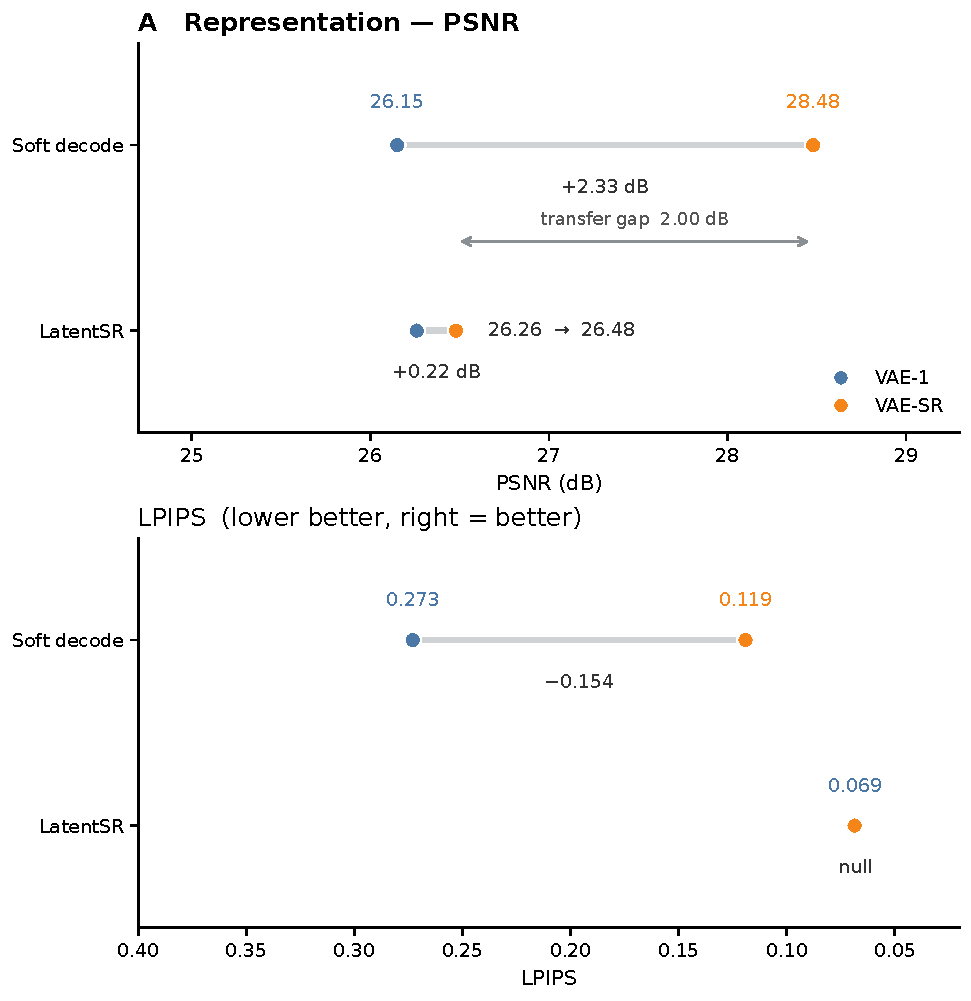
\includegraphics[width=\columnwidth]{figures/fig_a_representation.pdf}
  \caption{Representation vs.\ consumption, $n{=}64$.
  Soft-decode of $\zlr$ gains $+2.33$\,dB; concat \lsrmethod{} gains
  $+0.22$\,dB and LPIPS is a null (LPIPS axis reversed so better is
  right).}
  \label{fig:rep-gap}
\end{figure}

\begin{table}[H]
  \centering
  \caption{Matched concat / FiLM SR, $n{=}64$.
  Soft-decode is $\Dec(\zlr)$.}
  \label{tab:transfer}
  \small
  \begin{tabular}{@{}lcccc@{}}
    \toprule
     & soft PSNR & SR PSNR & soft LPIPS & SR LPIPS \\
    \midrule
    \vaeone{} concat & $26.15$ & $26.26$ & $0.273$ & $0.0683$ \\
    \vaesr{} concat & $\mathbf{28.48}$ & $26.48$ & $\mathbf{0.119}$ & $0.0685$ \\
    \vaesr{} FiLM & $28.48$ & $26.45$ & $0.119$ & $0.0696$ \\
    \bottomrule
  \end{tabular}
\end{table}

Paired tests on matched indices (\Cref{tab:paired}).
The concat $+0.22$\,dB is real and small; LPIPS is a null.
Secondary SSIM ($+0.0023$) and Sobel edge MAE ($-0.0028$) move with
PSNR.
Imagewise Spearman ($n{=}64$):
$\rho(\Delta\mathrm{PSNR}_{\mathrm{soft}},\Delta\mathrm{PSNR}_{\mathrm{SR}})=0.049$,
$\rho(\Delta\mathrm{LPIPS}_{\mathrm{soft}},\Delta\mathrm{LPIPS}_{\mathrm{SR}})=0.053$,
$\rho(\Delta\mathrm{PSNR}_{\mathrm{SR}},\mathrm{bicubic})= -0.139$,
$\rho(\Delta\mathrm{PSNR}_{\mathrm{SR}},\mathrm{HR\ Sobel})= +0.182$.
Images that gained the most in $\zlr$ did not gain more after
diffusion, so a $\lamal$ sweep is not the next question.
In latent space \vaesr{} shifts RMSE$(\zlr,\zhr)$ left while
RMSE$(\zsr,\zhr)$ overlaps \vaeone{}: the sampler lands in the same
neighborhood despite a better condition.

\subsection{Injection}
\label{sec:exp-film}

Spatial FiLM on the same frozen \vaesr{} does not close the gap
(\Cref{tab:transfer}, last row; \Cref{tab:paired}).
Train loss at epoch~$50$: concat $0.1333$ vs.\ FiLM $0.1343$
(val $0.1342$ vs.\ $0.1363$)---same plateau, FiLM slightly worse.
PSNR CI includes $0$; LPIPS is not a perceptual win.
Soft-decode is identical (same VAE).
FiLM+\vaeone{} was not trained (\S\ref{sec:method-film}).
The hole is not that the first convolution cannot see $\zlr$.

\begin{table}[H]
  \centering
  \caption{Paired tests, $n{=}64$.
  Concat row: \vaesr{} SR minus \vaeone{} SR.
  FiLM row: FiLM minus concat, both on \vaesr.}
  \label{tab:paired}
  \small
  \begin{tabular}{@{}llccc@{}}
    \toprule
    Contrast & Metric & $\Delta$ mean & $95\%$ CI & $p$ \\
    \midrule
    concat transfer & PSNR & $+0.217$ & $[+0.133,+0.300]$ & $10^{-4}$ \\
    concat transfer & LPIPS & $+0.0002$ & $[-0.0012,+0.0017]$ & $0.76$ \\
    FiLM vs.\ concat & PSNR & $-0.032$ & $[-0.089,+0.023]$ & $0.28$ \\
    FiLM vs.\ concat & LPIPS & $+0.0011$ & $[+0.0000,+0.0022]$ & $0.060$ \\
    \bottomrule
  \end{tabular}
\end{table}

\subsection{Reverse chain}
\label{sec:exp-traj}

\Cref{tab:cosine} and \Cref{fig:rev-chain} localize the miss.
\vaesr{} copies $\zlr$ mid-reverse ($\cos=\mathbf{0.985}$ at
$t{=}656$); \vaeone{} never does (peak $0.783$, coincidentally
\vaesr{}'s final number).
At $t{=}0$ most of the extra copy is gone ($0.615$ vs.\ $0.786$).
RMSE$(\zlr,\zhr)$ is constant in $t$: the VAEs differ; what changes
is the trajectory.
That is why concat and FiLM can both see a better code and still
emit nearly the same $\zsr$.

\begin{figure}[H]
  \centering
  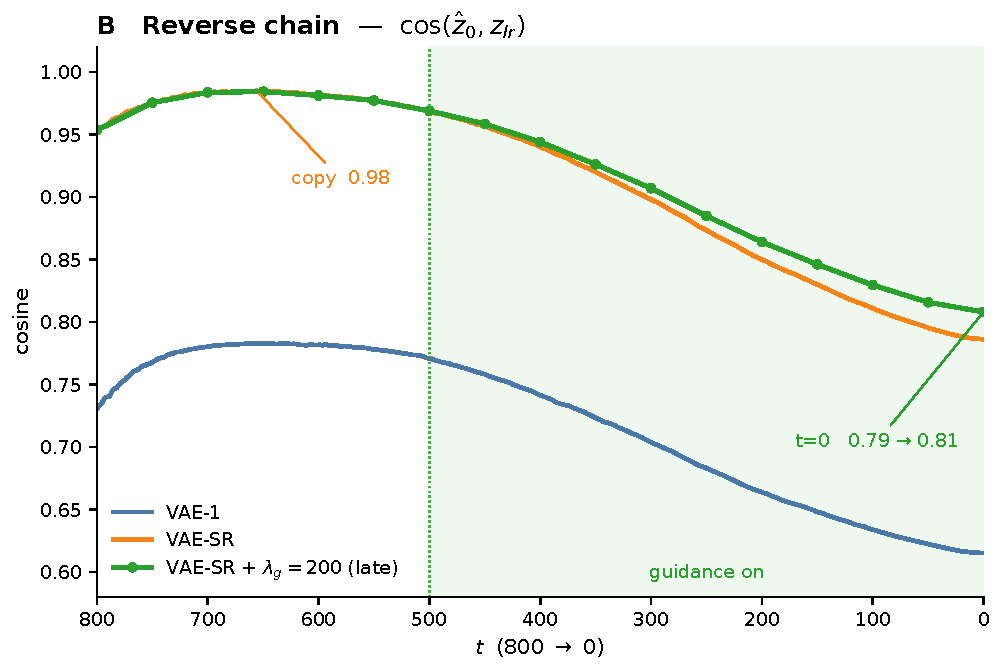
\includegraphics[width=\columnwidth]{figures/fig_b_reverse_chain.pdf}
  \caption{Reverse-chain cosine, $n{=}64$.
  \vaesr{} copies $\zlr$ near $t{=}656$ then the HR prior collapses
  the copy; late $\lamg{=}200$ ($t\le 500$) slows that collapse.}
  \label{fig:rev-chain}
\end{figure}

\begin{table}[H]
  \centering
  \caption{$\cos(\zhat(t),\zlr)$ along reverse sampling, $n{=}64$.}
  \label{tab:cosine}
  \small
  \begin{tabular}{@{}rcc@{}}
    \toprule
    $t$ & \vaeone{} & \vaesr{} \\
    \midrule
    $999$ (noise) & $0.282$ & $0.543$ \\
    $800$ & $0.730$ & $0.953$ \\
    $656$ (peak) & $0.783$ & $\mathbf{0.985}$ \\
    $500$ & $0.771$ & $0.969$ \\
    $400$ & $0.741$ & $0.940$ \\
    $0$ (clean) & $\mathbf{0.615}$ & $\mathbf{0.786}$ \\
    \bottomrule
  \end{tabular}
\end{table}

Latent cosine is not an image.
\Cref{tab:z0-img} decodes $\zhat(t)$ vs.\ $\xhr$; this is not
soft-decode $\Dec(\zlr)$.
Best absolute PSNR is near $t{=}400$ for both VAEs.
The $t{=}0$ $\Delta$ is exactly the concat $+0.22$\,dB.
Soft-decode $28.48$ is not $\Dec(\zhat)$ at the copy
($t{=}650$: $26.70$\,dB).

\begin{table}[H]
  \centering
  \caption{$\Dec(\zhat(t))$ vs.\ $\xhr$, $n{=}64$. Not soft-decode.}
  \label{tab:z0-img}
  \small
  \begin{tabular}{@{}rccc@{}}
    \toprule
    $t$ & PSNR \vaeone{} & PSNR \vaesr{} & $\Delta$ \\
    \midrule
    $800$ & $20.86$ & $22.64$ & $+1.78$ \\
    $650$ & $26.19$ & $26.70$ & $+0.51$ \\
    $400$ & $\mathbf{27.83}$ & $\mathbf{28.23}$ & $+0.39$ \\
    $0$ & $26.26$ & $26.48$ & $\mathbf{+0.22}$ \\
    \bottomrule
  \end{tabular}
\end{table}

\subsection{Guidance}
\label{sec:exp-guide}

Inference only: frozen \vaesr{} $+$ Q2 concat (\S\ref{sec:method-guide}).
Every job reprints $\mathrm{PSNR}(\Dec(\zlr),\xhr)=28.48$ on indices
$0..63$ or is discarded.

Stage~1 ($n{=}64$, $\lamg{=}200$): early $t\le 800$ and late
$t\le 500$ both reach $27.60$\,dB (\Cref{tab:stage1}).
All $64$ images gain PSNR.
LPIPS CIs include $0$ (early $p{=}0.29$, late $p{=}0.39$).
Trajectory moved: $t{=}0$ cosine $0.786\to 0.808$,
$\Lcal_g$ $0.00128\to 0.00048$---not a scale failure.
The windows tie to $0.003$\,dB; extra steps $t\in(500,800]$ lift
mid-chain $\Dec(\zhat)$ then late catches up by $t\approx 450$.
The finish comes from slowing the post-copy collapse ($t\le 500$).
Stage~2 is late-only; no combined schedule.

\begin{table}[H]
  \centering
  \caption{Stage~1 windows, $n{=}64$, $\lamg{=}200$.}
  \label{tab:stage1}
  \small
  \begin{tabular}{@{}lcc@{}}
    \toprule
    Method & PSNR & LPIPS \\
    \midrule
    Soft-decode (\vaesr) & $28.48$ & $0.119$ \\
    Unguided \lsrmethod{} & $26.48$ & $0.0685$ \\
    Early $t\le 800$ & $\mathbf{27.60}$ & $0.0695$ \\
    Late $t\le 500$ & $\mathbf{27.60}$ & $0.0693$ \\
    \bottomrule
  \end{tabular}
\end{table}

Stage~2, same $64$, late $t\le 500$, $\lamg\in\{50,200,800\}$
(\Cref{tab:dose64}, \Cref{fig:late-dose}).
Gap $28.482-26.478=\mathbf{2.004}$\,dB.
$\lamg{=}50$: smaller recon gain, LPIPS better on $\approx 80\%$ of
images.
$\lamg{=}200$: largest PSNR with no LPIPS tax---operating point.
$\lamg{=}800$: PSNR toward soft-decode, LPIPS toward $0.119$
(over-guidance).
$t{=}0$ cosine $0.786\to 0.794/0.808/0.837$: guidance does not lock
to the $0.985$ copy peak.

\Cref{tab:n256} is the pre-registered confirmation
(val\_index $0..255$, same checkpoints, late window).
Do not mix it with~\Cref{tab:dose64}.
Bars~\S\ref{sec:method-guide} all pass:
$255/256$ images gain PSNR at every $\lamg$ (sole miss:
\texttt{val\_index}~$99$, \texttt{162870.jpg});
$\Delta$LPIPS is monotone $50<200<800$;
all PSNR CIs exclude $0$.
Soft-decode on $256$ is $28.41$\,dB (first $64$ still $28.48$): extra
images, not a swapped VAE.
Gap $28.412-26.335=\mathbf{2.078}$\,dB; recovery $27\%/56\%/80\%$
matches $n{=}64$.
Unlike discovery, $\lamg{=}200$ LPIPS is significantly \emph{better}
than unguided ($p{=}0.0017$).
Operating point remains late $\lamg{=}200$: $26.33\to 27.50$\,dB
($56\%$ of the gap), LPIPS not walking to $0.119$.

\begin{figure}[H]
  \centering
  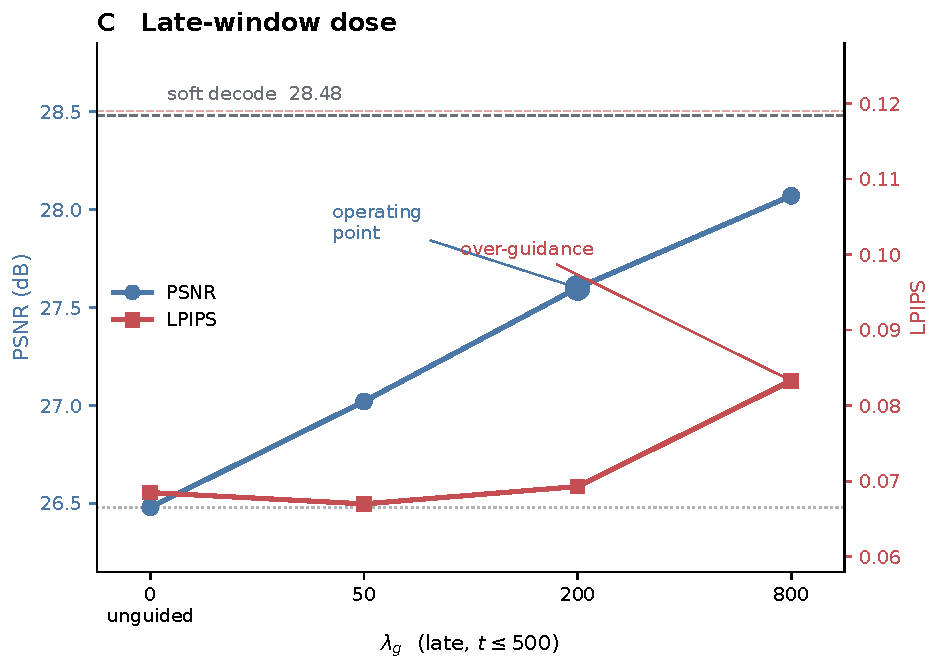
\includegraphics[width=\columnwidth,height=5.4cm,keepaspectratio]{figures/fig_c_late_dose.pdf}
  \caption{Late-window dose, $n{=}64$.
  $\lamg{=}200$ is the operating point; $\lamg{=}800$ walks LPIPS
  toward soft-decode $0.119$.
  Confirmatory $n{=}256$:~\Cref{tab:n256}.}
  \label{fig:late-dose}
\end{figure}

\begin{table}[H]
  \centering
  \caption{Late-window dose, $n{=}64$ (discovery).}
  \label{tab:dose64}
  \small
  \begin{tabular}{@{}lcccc@{}}
    \toprule
    $\lamg$ & PSNR & LPIPS & $\Delta$PSNR & $\%$ of gap \\
    \midrule
    $0$ & $26.48$ & $0.0685$ & --- & --- \\
    $50$ & $27.02$ & $\mathbf{0.0670}$ & $+0.54$ & $27\%$ \\
    $\mathbf{200}$ & $27.60$ & $0.0693$ & $+1.12$ & $\mathbf{56\%}$ \\
    $800$ & $28.07$ & $0.0833$ & $+1.59$ & $80\%$ \\
    soft-decode & $28.48$ & $0.119$ & $+2.00$ & $100\%$ \\
    \bottomrule
  \end{tabular}
\end{table}

\begin{table}[H]
  \centering
  \caption{Confirmatory late-window dose, $n{=}256$.
  $\Delta$ vs.\ unguided with $95\%$ CI.}
  \label{tab:n256}
  \small
  \begin{tabular}{@{}lcccc@{}}
    \toprule
    Method & PSNR & LPIPS & $\Delta$PSNR & $\%$ gap \\
    \midrule
    Soft-decode & $28.41$ & $0.119$ & --- & --- \\
    Unguided & $26.33$ & $0.0720$ & --- & --- \\
    Late $\lamg{=}50$ & $26.90$ & $\mathbf{0.0698}$ &
      \shortstack[l]{$+0.57$\\{\scriptsize $[0.53,0.60]$}} & $27\%$ \\
    Late $\lamg{=}200$ & $\mathbf{27.50}$ & $0.0707$ &
      \shortstack[l]{$+1.16$\\{\scriptsize $[1.11,1.22]$}} & $\mathbf{56\%}$ \\
    Late $\lamg{=}800$ & $28.00$ & $0.0832$ &
      \shortstack[l]{$+1.66$\\{\scriptsize $[1.60,1.72]$}} & $80\%$ \\
    \bottomrule
  \end{tabular}
\end{table}

\section{Discussion}
\label{sec:discussion}

The representation hypothesis is half right.
An SR-aware VAE really does improve $\zlr$:
soft-decode gains $+2.33$\,dB and LPIPS $0.273\to 0.119$ while HR
recon stays at $37.3$\,dB (\Cref{tab:vae-only}).
That improvement does not automatically become better SR.
Under a matched concat DDPM the SR PSNR gain is $+0.22$\,dB, LPIPS
is a null, and imagewise Spearman $\rho(\Delta\mathrm{soft},\Delta\mathrm{SR})\approx 0.05$
(\Cref{tab:transfer}, \Cref{tab:paired}).
Spatial FiLM on the same frozen \vaesr{} is also a PSNR null
(\Cref{tab:paired}).
The missing link is not ``the first convolution cannot read $\zlr$.''

The reverse-chain diagnostic is the more useful localization.
$\zhat(t)$ under \vaesr{} becomes strongly aligned with $\zlr$
mid-sampling (cosine $0.985$ at $t{=}656$) and then loses that
alignment by $t{=}0$ (\Cref{tab:cosine}, \Cref{fig:rev-chain}).
Decoding $\zhat(t)$ is not soft-decode: absolute PSNR peaks near
$t{=}400$, and the $t{=}0$ PSNR $\Delta$ matches the concat
$+0.22$\,dB (\Cref{tab:z0-img}).
We treat the late drop as an empirical fact about this reverse
process, not as a proof that an isolated ``HR prior'' is the cause.

Guidance tests that fact at inference, with no extra training.
Early and late windows at $\lamg{=}200$ tie
(\Cref{tab:stage1}): the finish is in $t\le 500$.
A late dose recovers $27\%/56\%/80\%$ of the transfer gap at
$\lamg\in\{50,200,800\}$; $\lamg{=}800$ walks LPIPS toward
soft-decode $0.119$ (\Cref{tab:dose64}, \Cref{fig:late-dose}).
The confirmatory table is $n{=}256$ (\Cref{tab:n256}):
late $\lamg{=}200$ moves $26.33\to 27.50$\,dB ($56\%$ of the
$2.08$\,dB gap) and slightly \emph{improves} LPIPS
($0.0720\to 0.0707$).
That is the operating point: recover a large share of the unused
representation gain without collapsing to the soft-decode image.

\paragraph{What we do not claim.}
This is not a new SR backbone, tokenizer, or trained guidance
network, and it is not a SOTA comparison against StableSR, SeeSR, or
DiffBIR.
The FiLM null is for this spatial conditioner on this frozen
\vaesr{} code; FiLM+\vaeone{} was not trained, so we do not claim a
VAE--conditioner interaction.
Soft-decode $\Dec(\zlr)$ is a probe of the condition, not an SR
method.
We do not claim that autoencoder quality transfers to SR in general.

\paragraph{Limits.}
The protocol is $4\times$ bicubic CelebA $32\to 128$ with a small
latent UNet trained from scratch.
VAE, concat, FiLM, and trajectory numbers are $n{=}64$; the
guidance dose we treat as confirmatory is $n{=}256$.
Guidance was not uniformly helpful: one image
(\texttt{val\_index}~$99$) had PSNR that worsened monotonically as
$\lamg$ increased, so the intervention is not failure-proof per
image even when the mean is strongly positive (\Cref{tab:n256}).
Full validation ($\approx 19{,}867$ images) is not run.
Guided sampling backpropagates through the frozen decoder at every
guided step and costs $\approx 21$\,s/image in our protocol
(\S\ref{sec:eval}), which is why the full split was infeasible.
We did not sweep $\lamal$.
Cosine$(\zlr,\zhr)$ plateaued after epoch~$1$ of the single
$\lamal{=}10^{-3}$ fine-tune (\S\ref{sec:method-vaesr}); that is a
training-curve observation, not a hyperparameter study, so we do not
claim $10^{-3}$ is optimal.
$\lamg{=}200$ is a compromise on $R(t)$, not a grid search over SR
PSNR.
A claimed related paper could not be verified from the citation as
given and was excluded (\S\ref{sec:setup-hygiene}).

The practical implication is narrow and, we think, useful.
If a better $\zlr$ does not move the SR table, the next experiment
is not necessarily a fancier injector.
Measure the reverse chain; if alignment appears and then fades,
inference-time decoder-side consistency on that window is a cheap
test of whether the unused information can still be spent.

\section{Conclusion}
\label{sec:conclusion}

Better LR latents need not yield better latent diffusion SR.
On a controlled CelebA $4\times$ protocol, an SR-aware VAE improves
soft-decode by $+2.33$\,dB, yet a matched concat DDPM---and spatial
FiLM on the same frozen code---consume almost none of that gain.
The reverse chain becomes strongly aligned with $\zlr$ mid-sampling
and then loses that alignment before $t{=}0$.
Decoder-side LR-consistency guidance on the late window, with no
extra training, recovers $56\%$ of the $2.08$\,dB transfer gap at
$\lamg{=}200$ ($n{=}256$: $26.33\to 27.50$\,dB) and slightly
improves LPIPS.
The contribution is that diagnosis and that inference-time test,
not a new SR architecture.


\section*{Code availability}
Training and evaluation code, configs, and the experiment log are at
\url{https://github.com/HusseinHanafy207/LatentSR}.
Paired checkpoints used in this report are at
\url{https://huggingface.co/HusseinHamouda/LatentSR-checkpoints}.

\bibliography{refs}

\end{document}
